\section{Protocolo Experimental, Parametrização e Resultados}
\label{sec:protocolo}

\subsection{Objetivo experimental}

O objetivo dos experimentos é comparar o ganho de custo dos métodos de melhoria (VND, GRASP fixo, GRASP reativo e Tabu) quando todos partem do mesmo baseline I1.
Para isso, a análise foi estruturada em dois níveis:
\begin{enumerate}
  \item calibração de parâmetros (\emph{tuning});
  \item execução comparativa consolidada em todas as instâncias de Solomon.
\end{enumerate}

\subsection{Etapas de validação e teste}
\label{subsec:etapas_validacao_teste}

Para tornar o processo reprodutível e auditável, a campanha experimental foi estruturada em etapas fixas.
Cada etapa tem uma entrada, uma checagem objetiva e um critério explícito de aprovação.

\begin{table}[htbp]
\centering
\caption{Checklist de validação e teste por etapa.}
\label{tab:validation_checklist}
\begin{tabular}{p{2.8cm}p{4.1cm}p{4.0cm}p{4.0cm}}
\hline
Etapa & Objetivo & Evidência gerada & Critério de aprovação \\
\hline
Build & Garantir compilação consistente do solver & Log de compilação e binário gerado & Compilar sem erro e sem quebra de linkagem \\
Validação estrutural & Confirmar formato da solução (depósito, cobertura, duplicidade) & Relatório de validação por instância & Todos os clientes atendidos exatamente uma vez \\
Validação de factibilidade & Confirmar restrições de capacidade e janelas de tempo & Recomputação das rotas e checagem de janelas/carga & Nenhuma violação de capacidade/janela \\
Validação de custo & Confirmar consistência da função objetivo & Custo total recomputado a partir das rotas & Custo reportado = custo recomputado \\
Teste funcional por algoritmo & Verificar execução fim-a-fim de I1, VND, GRASP e Tabu & CSV de execução + solução exportada & Execução concluída com solução factível \\
Teste comparativo & Medir qualidade relativa sob mesmo orçamento & Tabelas agregadas por instância e família & Comparação com mesma instância, seed e limite de tempo \\
\hline
\end{tabular}
\end{table}

\subsection{Desenho para seleção de vizinhanças}
\label{subsec:desenho_vizinhancas}

Como a seleção de vizinhanças afeta diretamente qualidade e custo computacional, recomenda-se uma sequência em três blocos:
\begin{enumerate}
  \item avaliação de cada vizinhança isoladamente;
  \item construção incremental (adição de operadores por ganho marginal);
  \item ablação (remoção de operadores a partir do conjunto completo).
\end{enumerate}

\begin{table}[htbp]
\centering
\caption{Plano de experimentos para seleção de vizinhanças.}
\label{tab:neighborhood_selection_plan}
\begin{tabular}{p{2.7cm}p{4.2cm}p{3.5cm}p{4.5cm}}
\hline
Bloco & Pergunta respondida & Configuração mínima & Critério de decisão \\
\hline
Isolado & ``Esta vizinhança é forte sozinha?'' & 1 vizinhança ativa por execução & Manter candidatas com ganho consistente de custo \\
Incremental & ``Quanto essa vizinhança agrega ao conjunto atual?'' & Adição uma a uma sobre baseline fixo & Priorizar maior ganho marginal por segundo \\
Ablativo & ``O que acontece se eu retirar esta vizinhança?'' & Conjunto completo menos 1 operador & Remover operadores com baixo impacto e alto custo \\
Confirmação & ``A seleção generaliza fora do tuning?'' & Repetição no teste final (holdout) & Seleção válida se mantém ranking em famílias C/R/RC \\
\hline
\end{tabular}
\end{table}

\subsection{Configuração operacional da seleção de vizinhanças}
\label{subsec:config_operacional_vizinhancas}

A seleção de vizinhanças é executada com um motor dedicado de busca local (\texttt{nls}), sem relacionar os resultados com GRASP ou Tabu nesta etapa.
A configuração base é:
\begin{itemize}
  \item solução inicial fixa em Solomon I1;
  \item política \emph{first improvement} em todas as vizinhanças;
  \item Fase A com \texttt{nls\_restart = 0} (triagem isolada sem reinício);
  \item Fase B com \texttt{nls\_restart = 1}, em que subconjuntos com múltiplas vizinhanças são executados no esquema clássico de VND (ordem por complexidade e reinício na primeira vizinhança ao melhorar);
  \item validação completa de factibilidade (capacidade, janelas de tempo e cobertura de clientes) ao final de cada execução.
\end{itemize}

\begin{table}[htbp]
\centering
\caption{Variáveis registradas por instância e configuração durante a seleção de vizinhanças.}
\label{tab:neighborhood_selection_variables}
\begin{tabular}{p{3.3cm}p{5.0cm}p{5.0cm}}
\hline
Variável & Significado & Uso na decisão \\
\hline
\texttt{cost} & Custo real final da solução factível & Comparação nominal e cálculo de gap \\
\texttt{num\_routes} & Número de veículos (rotas não triviais) & Verificação de impacto na frota \\
\texttt{time\_sec} & Tempo de execução da configuração na instância & Desempate por custo computacional \\
\texttt{gap\_pct} & Gap percentual em relação ao BKS & Métrica primária para ranking \\
\hline
\end{tabular}
\end{table}

\subsection{Plano estatístico e critérios de reporte}
\label{subsec:plano_estatistico}

Para reduzir risco de conclusões por ruído, a análise final deve combinar medidas de tendência central, dispersão e testes não paramétricos por instância.

\begin{table}[htbp]
\centering
\caption{Plano mínimo de análise estatística para comparação de métodos.}
\label{tab:statistical_plan}
\begin{tabular}{p{3.2cm}p{3.8cm}p{3.7cm}p{3.8cm}}
\hline
Componente & Prática recomendada & Resultado reportado & Decisão \\
\hline
Métrica primária & Gap (\%) por instância e seed & Mediana, média e desvio padrão & Ranking principal por mediana de gap \\
Métrica secundária & Custo nominal, veículos e tempo & Tabelas por instância/família & Verificar trade-off custo vs frota vs tempo \\
Teste de hipótese (par a par) & Wilcoxon signed-rank (instância a instância) & $p$-valor + direção da diferença & Confirmar se ganho é estatisticamente robusto \\
Múltiplos algoritmos & Friedman + pós-teste de Nemenyi (ou Holm) & Ranking médio + grupos sem diferença & Evitar conclusão com múltiplas comparações sem controle \\
Tamanho de efeito & Cliff's delta ou diferença mediana & Magnitude do efeito & Distinguir diferença prática de diferença pequena \\
\hline
\end{tabular}
\end{table}

\paragraph{Síntese metodológica.}
A estratégia ``isolado + incremental + ablação + confirmação'' é adequada para seleção de vizinhanças em meta-heurísticas, pois separa contribuição individual, sinergia e custo computacional.
Do ponto de vista de metodologia científica, essa abordagem é forte quando executada com:
\begin{itemize}
  \item orçamento de tempo idêntico entre métodos;
  \item múltiplas seeds;
  \item separação entre tuning e teste final;
  \item reporte de incerteza e teste estatístico.
\end{itemize}

\subsection{Calibração de seeds e tempo-limite}
\label{subsec:calibracao_seed_tempo}

As escolhas de \texttt{seed} e \texttt{time-limit} não devem ser arbitrárias: elas definem o nível de variabilidade observada e a justiça da comparação entre métodos \cite{barr1995experiments,hooker1995testing}.

\subsubsection{Critério para número de seeds}

Para algoritmos estocásticos, recomenda-se calibrar o número de seeds por estudo piloto incremental, em linha com boas práticas de desenho experimental e reporte de heurísticas \cite{barr1995experiments,hooker1995testing}:
\[
n \in \{3,5,7,10,15,20\}.
\]
Em cada $n$, estima-se a estabilidade de ranking e a incerteza da métrica primária (gap). O menor $n$ aceito deve satisfazer simultaneamente:
\begin{itemize}
  \item correlação de ranking (Spearman) com a referência $n=20$ maior ou igual a 0.95 \cite{demsar2006statistical};
  \item semi-amplitude do IC95\% da mediana do gap abaixo do limiar definido no protocolo (ex.: 0.5 p.p.).
\end{itemize}

Para métodos determinísticos, uma seed é suficiente para execução, mas deve-se manter o mesmo conjunto de instâncias e orçamento para comparabilidade com os métodos estocásticos.

\subsubsection{Critério para tempo-limite}

O \texttt{time-limit} deve ser calibrado por instância (ou por família) a partir de uma referência fixa.
Uma forma robusta é usar o tempo mediano de um baseline determinístico e aplicar um multiplicador:
\[
T_i = \min\{T_{\max},\max[T_{\min},\kappa\cdot t^{ref}_i]\},
\]
em que $t^{ref}_i$ é o tempo da referência na instância $i$ (mediano no piloto), e $\kappa$ controla o orçamento.
Na comparação final, todos os algoritmos recebem o mesmo $T_i$ na mesma instância.

\subsubsection{Recomendação prática para este trabalho}

No pipeline atual, os valores usados como ponto de partida foram:
\begin{itemize}
  \item tuning: seeds 42--46;
  \item campanha consolidada: seeds 42--51.
\end{itemize}
Esses valores são aceitáveis como baseline operacional, mas devem ser validados pelo procedimento piloto acima para justificar rigor metodológico no relatório final.
Para calibração automática de parâmetros, manter esse desenho desacoplado do \emph{racing} do \texttt{irace} evita enviesar a avaliação \cite{lopez2016irace}.

\IfFileExists{tables/seed_time_calibration_template.tex}{
\begin{table}[htbp]
\centering
\caption{Piloto para calibração do número de seeds.}
\label{tab:seed_calibration_template}
\begin{tabular}{lrrrrr}
\hline
$n$ seeds & Instâncias & Mediana gap (\%) & IC95\% semi-amplitude & Spearman vs $n=20$ & Decisão \\
\hline
3  &  &  &  &  &  \\
5  &  &  &  &  &  \\
7  &  &  &  &  &  \\
10 &  &  &  &  &  \\
15 &  &  &  &  &  \\
20 &  &  &  & 1.000 & Referência \\
\hline
\end{tabular}
\end{table}

\begin{table}[htbp]
\centering
\caption{Piloto para calibração de tempo-limite por instância/família.}
\label{tab:time_calibration_template}
\begin{tabular}{lrrrrrr}
\hline
Grupo & $t^{ref}$ mediano (s) & $\kappa$ & $T_{\min}$ & $T_{\max}$ & $T_i$ aplicado (s) & Observação \\
\hline
C  &  &  &  &  &  &  \\
R  &  &  &  &  &  &  \\
RC &  &  &  &  &  &  \\
\hline
\end{tabular}
\end{table}

\begin{table}[htbp]
\centering
\caption{Resumo final do protocolo de seeds e tempo para os experimentos.}
\label{tab:seed_time_final_protocol}
\begin{tabular}{llll}
\hline
Fase & Seeds adotadas & Regra de tempo & Critério de aceite \\
\hline
Tuning &  &  &  \\
Comparação final &  &  &  \\
\hline
\end{tabular}
\end{table}

}{
\begin{table}[htbp]
\centering
\caption{Template de calibração de seeds e tempo-limite (pendente).}
\begin{tabular}{lc}
\hline
Status & Observação \\
\hline
Pendente & Preencher \texttt{tables/seed\_time\_calibration\_template.tex} após estudo piloto. \\
\hline
\end{tabular}
\end{table}
}

\subsection{Instâncias e métricas}

As instâncias pertencem ao benchmark clássico de Solomon \cite{solomon1987algorithms}, cobrindo famílias C, R e RC.

A métrica primária é o gap percentual em relação ao BKS:
\[
\text{gap}(\%) = 100\cdot\left(\frac{cost}{BKS}-1\right).
\]

Além do gap, este trabalho reporta:
\begin{itemize}
  \item custo nominal da solução;
  \item número de veículos;
  \item variação de veículos por algoritmo em relação ao BKS.
\end{itemize}

Para a variação de veículos por instância $i$ e algoritmo $a$, usa-se:
\[
\Delta veh_{a,i} = veh_{a,i} - veh^{BKS}_{i}.
\]
Valores negativos indicam redução de frota em relação ao melhor valor conhecido.

\subsection{Parametrização adotada}

\subsubsection{Parâmetros fixos de alinhamento}

Para preservar comparabilidade metodológica, o construtivo base foi fixado na forma clássica orientada à distância:
\[
\alpha_1=1,\;\alpha_2=0,\;\lambda=1,\;\mu=1.
\]

No solver, tentativas de executar com $\mu\neq 1$ são explicitamente rejeitadas.

\subsubsection{Parâmetros por algoritmo}

\begin{itemize}
  \item \textbf{VND}: conjunto fixo das quatro vizinhanças selecionadas;
  \item \textbf{GRASP fixo}: $\alpha$ fixo;
  \item \textbf{GRASP reativo}: conjunto de $\alpha$, frequência de atualização e $\gamma$;
  \item \textbf{Tabu}: tenure, limite de iterações e limite sem melhoria.
\end{itemize}

\subsection{Calibração com \emph{irace}}

A calibração automática foi definida com \emph{irace} \cite{lopez2016irace} em tuning set separado.
O espaço de busca inclui:
\begin{itemize}
  \item \textbf{Tabu}: \texttt{tenure}, \texttt{max\_iters}, \texttt{max\_no\_improve};
  \item \textbf{GRASP reativo}: \texttt{reactive\_update}, \texttt{reactive\_gamma}, conjunto de \texttt{reactive\_alphas}, \texttt{max\_iters}, \texttt{max\_no\_improve}.
\end{itemize}

O processo completo de calibração e reprodutibilidade está documentado em \texttt{docs/calibration\_process\_irace.md}.

\subsection{Tabelas completas por algoritmo}
\label{subsec:tabelas_por_algoritmo}

Para manter legibilidade e ainda preservar todos os resultados das 56 instâncias, os dados foram organizados em tabelas separadas por algoritmo.
Em todas elas, cada linha é uma instância e as colunas são:
\begin{itemize}
  \item custo real;
  \item $\Delta$custo em relação ao BKS;
  \item gap (\%) em relação ao BKS;
  \item número de veículos;
  \item $\Delta$veículos em relação ao BKS;
  \item tempo de execução (s).
\end{itemize}

Nas tabelas de GRASP e Tabu, inclui-se também a coluna de iterações executadas.

\IfFileExists{tables/instance_tables_by_algorithm.tex}{
% Auto-generated by scripts/build_algorithm_tables_and_summary.py
\ifdefined\longtable
\scriptsize
\begin{longtable}{lrrrrrr}
\caption{Resultados por instancia para I1 (\texttt{i1}).}\label{tab:inst-i1}\\
\hline
Instancia & custo & $\Delta$custo(BKS) & gap(\%) & veiculos & $\Delta$veiculos(BKS) & tempo(s) \\
\hline
\endfirsthead
\hline
Instancia & custo & $\Delta$custo(BKS) & gap(\%) & veiculos & $\Delta$veiculos(BKS) & tempo(s) \\
\hline
\endhead
C101 & 922.0 & 94.7 & 11.45 & 10.00 & 0.00 & 0.072 \\
C102 & 1113.4 & 286.1 & 34.58 & 11.00 & 1.00 & 0.049 \\
C103 & 1165.9 & 339.6 & 41.10 & 11.00 & 1.00 & 0.032 \\
C104 & 1156.4 & 333.5 & 40.53 & 10.00 & 0.00 & 0.092 \\
C105 & 877.0 & 49.7 & 6.01 & 10.00 & 0.00 & 0.048 \\
C106 & 949.9 & 122.6 & 14.82 & 11.00 & 1.00 & 0.031 \\
C107 & 926.9 & 99.6 & 12.04 & 10.00 & 0.00 & 0.061 \\
C108 & 945.1 & 117.8 & 14.24 & 10.00 & 0.00 & 0.056 \\
C109 & 940.6 & 113.3 & 13.70 & 10.00 & 0.00 & 0.106 \\
C201 & 609.1 & 20.0 & 3.40 & 3.00 & 0.00 & 0.186 \\
C202 & 806.3 & 217.2 & 36.87 & 4.00 & 1.00 & 0.200 \\
C203 & 743.0 & 154.3 & 26.21 & 4.00 & 1.00 & 0.323 \\
C204 & 1001.5 & 413.4 & 70.29 & 4.00 & 1.00 & 0.098 \\
C205 & 706.2 & 119.8 & 20.43 & 4.00 & 1.00 & 0.302 \\
C206 & 696.8 & 110.8 & 18.91 & 4.00 & 1.00 & 0.186 \\
C207 & 680.5 & 94.7 & 16.17 & 3.00 & 0.00 & 0.227 \\
C208 & 686.4 & 100.6 & 17.17 & 3.00 & 0.00 & 0.211 \\
R101 & 1826.0 & 188.3 & 11.50 & 21.00 & 1.00 & 0.111 \\
R102 & 1797.2 & 330.6 & 22.54 & 19.00 & 1.00 & 0.144 \\
R103 & 1473.2 & 264.5 & 21.88 & 16.00 & 2.00 & 0.086 \\
R104 & 1262.3 & 290.8 & 29.93 & 12.00 & 1.00 & 0.148 \\
R105 & 1681.0 & 325.7 & 24.03 & 16.00 & 1.00 & 0.065 \\
R106 & 1437.7 & 203.1 & 16.45 & 14.00 & 1.00 & 0.059 \\
R107 & 1317.8 & 253.2 & 23.78 & 12.00 & 1.00 & 0.110 \\
R108 & 1180.1 & 248.0 & 26.61 & 11.00 & 1.00 & 0.140 \\
R109 & 1415.4 & 268.5 & 23.41 & 14.00 & 1.00 & 0.189 \\
R110 & 1313.9 & 245.9 & 23.02 & 12.00 & 0.00 & 0.064 \\
R111 & 1267.1 & 218.4 & 20.83 & 13.00 & 1.00 & 0.116 \\
R112 & 1198.9 & 250.3 & 26.39 & 11.00 & 1.00 & 0.076 \\
R201 & 1849.3 & 706.1 & 61.77 & 5.00 & -3.00 & 0.088 \\
R202 & 1612.6 & 583.0 & 56.62 & 4.00 & -4.00 & 0.183 \\
R203 & 1473.2 & 602.4 & 69.18 & 4.00 & -2.00 & 0.300 \\
R204 & 1129.6 & 398.3 & 54.46 & 3.00 & -2.00 & 0.233 \\
R205 & 1451.0 & 501.2 & 52.77 & 4.00 & -1.00 & 0.225 \\
R206 & 1380.8 & 504.9 & 57.64 & 3.00 & -2.00 & 0.396 \\
R207 & 1192.8 & 398.8 & 50.23 & 3.00 & -1.00 & 0.269 \\
R208 & 926.4 & 225.4 & 32.15 & 3.00 & -1.00 & 0.226 \\
R209 & 1325.1 & 470.3 & 55.02 & 4.00 & -1.00 & 0.229 \\
R210 & 1332.1 & 431.6 & 47.93 & 4.00 & -2.00 & 0.273 \\
R211 & 1126.8 & 380.1 & 50.90 & 3.00 & -1.00 & 0.222 \\
RC101 & 1962.1 & 342.3 & 21.13 & 17.00 & 2.00 & 0.133 \\
RC102 & 1627.5 & 170.1 & 11.67 & 15.00 & 1.00 & 0.173 \\
RC103 & 1546.9 & 288.9 & 22.97 & 13.00 & 2.00 & 0.103 \\
RC104 & 1333.7 & 201.4 & 17.79 & 12.00 & 2.00 & 0.078 \\
RC105 & 1793.2 & 279.5 & 18.46 & 17.00 & 2.00 & 0.191 \\
RC106 & 1615.3 & 242.6 & 17.67 & 14.00 & 2.00 & 0.167 \\
RC107 & 1431.9 & 224.1 & 18.55 & 13.00 & 1.00 & 0.115 \\
RC108 & 1326.2 & 212.0 & 19.03 & 12.00 & 1.00 & 0.122 \\
RC201 & 1972.4 & 710.6 & 56.32 & 5.00 & -4.00 & 0.187 \\
RC202 & 1996.5 & 904.2 & 82.78 & 5.00 & -3.00 & 0.174 \\
RC203 & 1626.5 & 702.8 & 76.09 & 4.00 & -1.00 & 0.131 \\
RC204 & 1284.7 & 501.2 & 63.97 & 4.00 & 0.00 & 0.235 \\
RC205 & 1904.3 & 750.3 & 65.02 & 5.00 & -2.00 & 0.207 \\
RC206 & 1943.7 & 892.6 & 84.92 & 4.00 & -3.00 & 0.176 \\
RC207 & 1733.5 & 770.6 & 80.03 & 4.00 & -2.00 & 0.101 \\
RC208 & 1235.7 & 459.6 & 59.22 & 3.00 & -1.00 & 0.260 \\
\hline
\end{longtable}
\else
\begin{table}[p]
\centering
\scriptsize
\caption{Resultados por instancia para I1 (\texttt{i1}).}
\label{tab:inst-i1}
\begin{tabular}{lrrrrrr}
\hline
Instancia & custo & $\Delta$custo(BKS) & gap(\%) & veiculos & $\Delta$veiculos(BKS) & tempo(s) \\
\hline
C101 & 922.0 & 94.7 & 11.45 & 10.00 & 0.00 & 0.072 \\
C102 & 1113.4 & 286.1 & 34.58 & 11.00 & 1.00 & 0.049 \\
C103 & 1165.9 & 339.6 & 41.10 & 11.00 & 1.00 & 0.032 \\
C104 & 1156.4 & 333.5 & 40.53 & 10.00 & 0.00 & 0.092 \\
C105 & 877.0 & 49.7 & 6.01 & 10.00 & 0.00 & 0.048 \\
C106 & 949.9 & 122.6 & 14.82 & 11.00 & 1.00 & 0.031 \\
C107 & 926.9 & 99.6 & 12.04 & 10.00 & 0.00 & 0.061 \\
C108 & 945.1 & 117.8 & 14.24 & 10.00 & 0.00 & 0.056 \\
C109 & 940.6 & 113.3 & 13.70 & 10.00 & 0.00 & 0.106 \\
C201 & 609.1 & 20.0 & 3.40 & 3.00 & 0.00 & 0.186 \\
C202 & 806.3 & 217.2 & 36.87 & 4.00 & 1.00 & 0.200 \\
C203 & 743.0 & 154.3 & 26.21 & 4.00 & 1.00 & 0.323 \\
C204 & 1001.5 & 413.4 & 70.29 & 4.00 & 1.00 & 0.098 \\
C205 & 706.2 & 119.8 & 20.43 & 4.00 & 1.00 & 0.302 \\
C206 & 696.8 & 110.8 & 18.91 & 4.00 & 1.00 & 0.186 \\
C207 & 680.5 & 94.7 & 16.17 & 3.00 & 0.00 & 0.227 \\
C208 & 686.4 & 100.6 & 17.17 & 3.00 & 0.00 & 0.211 \\
R101 & 1826.0 & 188.3 & 11.50 & 21.00 & 1.00 & 0.111 \\
R102 & 1797.2 & 330.6 & 22.54 & 19.00 & 1.00 & 0.144 \\
R103 & 1473.2 & 264.5 & 21.88 & 16.00 & 2.00 & 0.086 \\
R104 & 1262.3 & 290.8 & 29.93 & 12.00 & 1.00 & 0.148 \\
R105 & 1681.0 & 325.7 & 24.03 & 16.00 & 1.00 & 0.065 \\
R106 & 1437.7 & 203.1 & 16.45 & 14.00 & 1.00 & 0.059 \\
R107 & 1317.8 & 253.2 & 23.78 & 12.00 & 1.00 & 0.110 \\
R108 & 1180.1 & 248.0 & 26.61 & 11.00 & 1.00 & 0.140 \\
R109 & 1415.4 & 268.5 & 23.41 & 14.00 & 1.00 & 0.189 \\
R110 & 1313.9 & 245.9 & 23.02 & 12.00 & 0.00 & 0.064 \\
R111 & 1267.1 & 218.4 & 20.83 & 13.00 & 1.00 & 0.116 \\
R112 & 1198.9 & 250.3 & 26.39 & 11.00 & 1.00 & 0.076 \\
R201 & 1849.3 & 706.1 & 61.77 & 5.00 & -3.00 & 0.088 \\
R202 & 1612.6 & 583.0 & 56.62 & 4.00 & -4.00 & 0.183 \\
R203 & 1473.2 & 602.4 & 69.18 & 4.00 & -2.00 & 0.300 \\
R204 & 1129.6 & 398.3 & 54.46 & 3.00 & -2.00 & 0.233 \\
R205 & 1451.0 & 501.2 & 52.77 & 4.00 & -1.00 & 0.225 \\
R206 & 1380.8 & 504.9 & 57.64 & 3.00 & -2.00 & 0.396 \\
R207 & 1192.8 & 398.8 & 50.23 & 3.00 & -1.00 & 0.269 \\
R208 & 926.4 & 225.4 & 32.15 & 3.00 & -1.00 & 0.226 \\
R209 & 1325.1 & 470.3 & 55.02 & 4.00 & -1.00 & 0.229 \\
R210 & 1332.1 & 431.6 & 47.93 & 4.00 & -2.00 & 0.273 \\
R211 & 1126.8 & 380.1 & 50.90 & 3.00 & -1.00 & 0.222 \\
RC101 & 1962.1 & 342.3 & 21.13 & 17.00 & 2.00 & 0.133 \\
RC102 & 1627.5 & 170.1 & 11.67 & 15.00 & 1.00 & 0.173 \\
RC103 & 1546.9 & 288.9 & 22.97 & 13.00 & 2.00 & 0.103 \\
RC104 & 1333.7 & 201.4 & 17.79 & 12.00 & 2.00 & 0.078 \\
RC105 & 1793.2 & 279.5 & 18.46 & 17.00 & 2.00 & 0.191 \\
RC106 & 1615.3 & 242.6 & 17.67 & 14.00 & 2.00 & 0.167 \\
RC107 & 1431.9 & 224.1 & 18.55 & 13.00 & 1.00 & 0.115 \\
RC108 & 1326.2 & 212.0 & 19.03 & 12.00 & 1.00 & 0.122 \\
RC201 & 1972.4 & 710.6 & 56.32 & 5.00 & -4.00 & 0.187 \\
RC202 & 1996.5 & 904.2 & 82.78 & 5.00 & -3.00 & 0.174 \\
RC203 & 1626.5 & 702.8 & 76.09 & 4.00 & -1.00 & 0.131 \\
RC204 & 1284.7 & 501.2 & 63.97 & 4.00 & 0.00 & 0.235 \\
RC205 & 1904.3 & 750.3 & 65.02 & 5.00 & -2.00 & 0.207 \\
RC206 & 1943.7 & 892.6 & 84.92 & 4.00 & -3.00 & 0.176 \\
RC207 & 1733.5 & 770.6 & 80.03 & 4.00 & -2.00 & 0.101 \\
RC208 & 1235.7 & 459.6 & 59.22 & 3.00 & -1.00 & 0.260 \\
\hline
\end{tabular}
\end{table}
\fi

\ifdefined\longtable
\scriptsize
\begin{longtable}{lrrrrrr}
\caption{Resultados por instancia para VND (\texttt{vnd}).}\label{tab:inst-vnd}\\
\hline
Instancia & custo & $\Delta$custo(BKS) & gap(\%) & veiculos & $\Delta$veiculos(BKS) & tempo(s) \\
\hline
\endfirsthead
\hline
Instancia & custo & $\Delta$custo(BKS) & gap(\%) & veiculos & $\Delta$veiculos(BKS) & tempo(s) \\
\hline
\endhead
C101 & 827.3 & 0.0 & 0.00 & 10.00 & 0.00 & 0.145 \\
C102 & 919.9 & 92.6 & 11.19 & 11.00 & 1.00 & 0.384 \\
C103 & 1000.3 & 174.0 & 21.06 & 11.00 & 1.00 & 0.511 \\
C104 & 1010.0 & 187.1 & 22.74 & 10.00 & 0.00 & 0.441 \\
C105 & 827.3 & 0.0 & 0.00 & 10.00 & 0.00 & 0.086 \\
C106 & 851.3 & 24.0 & 2.90 & 11.00 & 1.00 & 0.110 \\
C107 & 827.3 & 0.0 & 0.00 & 10.00 & 0.00 & 0.220 \\
C108 & 827.3 & 0.0 & 0.00 & 10.00 & 0.00 & 0.108 \\
C109 & 847.5 & 20.2 & 2.44 & 10.00 & 0.00 & 0.284 \\
C201 & 589.1 & 0.0 & 0.00 & 3.00 & 0.00 & 0.129 \\
C202 & 620.9 & 31.8 & 5.40 & 4.00 & 1.00 & 0.772 \\
C203 & 619.7 & 31.0 & 5.27 & 4.00 & 1.00 & 0.257 \\
C204 & 756.0 & 167.9 & 28.55 & 4.00 & 1.00 & 0.333 \\
C205 & 609.3 & 22.9 & 3.91 & 4.00 & 1.00 & 0.501 \\
C206 & 614.1 & 28.1 & 4.80 & 4.00 & 1.00 & 0.302 \\
C207 & 585.8 & 0.0 & 0.00 & 3.00 & 0.00 & 0.552 \\
C208 & 585.8 & 0.0 & 0.00 & 3.00 & 0.00 & 0.384 \\
R101 & 1693.3 & 55.6 & 3.40 & 21.00 & 1.00 & 0.276 \\
R102 & 1524.5 & 57.9 & 3.95 & 19.00 & 1.00 & 0.831 \\
R103 & 1320.4 & 111.7 & 9.24 & 16.00 & 2.00 & 0.241 \\
R104 & 1122.6 & 151.1 & 15.55 & 12.00 & 1.00 & 0.547 \\
R105 & 1495.1 & 139.8 & 10.32 & 16.00 & 1.00 & 0.193 \\
R106 & 1320.9 & 86.3 & 6.99 & 14.00 & 1.00 & 0.195 \\
R107 & 1221.1 & 156.5 & 14.70 & 12.00 & 1.00 & 0.371 \\
R108 & 1089.5 & 157.4 & 16.89 & 11.00 & 1.00 & 0.450 \\
R109 & 1312.1 & 165.2 & 14.40 & 14.00 & 1.00 & 0.288 \\
R110 & 1249.4 & 181.4 & 16.99 & 12.00 & 0.00 & 0.155 \\
R111 & 1148.7 & 100.0 & 9.54 & 13.00 & 1.00 & 0.205 \\
R112 & 1045.2 & 96.6 & 10.18 & 11.00 & 1.00 & 0.248 \\
R201 & 1239.7 & 96.5 & 8.44 & 5.00 & -3.00 & 0.284 \\
R202 & 1196.5 & 166.9 & 16.21 & 4.00 & -4.00 & 0.916 \\
R203 & 991.0 & 120.2 & 13.80 & 4.00 & -2.00 & 1.311 \\
R204 & 927.4 & 196.1 & 26.82 & 3.00 & -2.00 & 1.049 \\
R205 & 1132.8 & 183.0 & 19.27 & 4.00 & -1.00 & 0.567 \\
R206 & 1122.4 & 246.5 & 28.14 & 3.00 & -2.00 & 0.632 \\
R207 & 908.7 & 114.7 & 14.45 & 3.00 & -1.00 & 1.222 \\
R208 & 795.8 & 94.8 & 13.52 & 3.00 & -1.00 & 0.761 \\
R209 & 1095.3 & 240.5 & 28.14 & 4.00 & -1.00 & 0.286 \\
R210 & 961.1 & 60.6 & 6.73 & 4.00 & -2.00 & 0.870 \\
R211 & 902.2 & 155.5 & 20.82 & 3.00 & -1.00 & 0.716 \\
RC101 & 1744.4 & 124.6 & 7.69 & 17.00 & 2.00 & 0.230 \\
RC102 & 1552.4 & 95.0 & 6.52 & 15.00 & 1.00 & 0.136 \\
RC103 & 1395.3 & 137.3 & 10.91 & 13.00 & 2.00 & 0.403 \\
RC104 & 1220.7 & 88.4 & 7.81 & 12.00 & 2.00 & 0.329 \\
RC105 & 1676.3 & 162.6 & 10.74 & 17.00 & 2.00 & 0.289 \\
RC106 & 1476.3 & 103.6 & 7.55 & 14.00 & 2.00 & 0.391 \\
RC107 & 1336.4 & 128.6 & 10.65 & 13.00 & 1.00 & 0.384 \\
RC108 & 1235.7 & 121.5 & 10.90 & 12.00 & 1.00 & 0.305 \\
RC201 & 1513.6 & 251.8 & 19.96 & 5.00 & -4.00 & 0.627 \\
RC202 & 1316.9 & 224.6 & 20.56 & 5.00 & -3.00 & 0.923 \\
RC203 & 1105.1 & 181.4 & 19.64 & 4.00 & -1.00 & 0.624 \\
RC204 & 927.1 & 143.6 & 18.33 & 4.00 & 0.00 & 0.828 \\
RC205 & 1395.8 & 241.8 & 20.95 & 5.00 & -2.00 & 0.935 \\
RC206 & 1372.0 & 320.9 & 30.53 & 4.00 & -3.00 & 0.958 \\
RC207 & 1270.9 & 308.0 & 31.99 & 4.00 & -2.00 & 0.699 \\
RC208 & 1084.0 & 307.9 & 39.67 & 3.00 & -1.00 & 0.541 \\
\hline
\end{longtable}
\else
\begin{table}[p]
\centering
\scriptsize
\caption{Resultados por instancia para VND (\texttt{vnd}).}
\label{tab:inst-vnd}
\begin{tabular}{lrrrrrr}
\hline
Instancia & custo & $\Delta$custo(BKS) & gap(\%) & veiculos & $\Delta$veiculos(BKS) & tempo(s) \\
\hline
C101 & 827.3 & 0.0 & 0.00 & 10.00 & 0.00 & 0.145 \\
C102 & 919.9 & 92.6 & 11.19 & 11.00 & 1.00 & 0.384 \\
C103 & 1000.3 & 174.0 & 21.06 & 11.00 & 1.00 & 0.511 \\
C104 & 1010.0 & 187.1 & 22.74 & 10.00 & 0.00 & 0.441 \\
C105 & 827.3 & 0.0 & 0.00 & 10.00 & 0.00 & 0.086 \\
C106 & 851.3 & 24.0 & 2.90 & 11.00 & 1.00 & 0.110 \\
C107 & 827.3 & 0.0 & 0.00 & 10.00 & 0.00 & 0.220 \\
C108 & 827.3 & 0.0 & 0.00 & 10.00 & 0.00 & 0.108 \\
C109 & 847.5 & 20.2 & 2.44 & 10.00 & 0.00 & 0.284 \\
C201 & 589.1 & 0.0 & 0.00 & 3.00 & 0.00 & 0.129 \\
C202 & 620.9 & 31.8 & 5.40 & 4.00 & 1.00 & 0.772 \\
C203 & 619.7 & 31.0 & 5.27 & 4.00 & 1.00 & 0.257 \\
C204 & 756.0 & 167.9 & 28.55 & 4.00 & 1.00 & 0.333 \\
C205 & 609.3 & 22.9 & 3.91 & 4.00 & 1.00 & 0.501 \\
C206 & 614.1 & 28.1 & 4.80 & 4.00 & 1.00 & 0.302 \\
C207 & 585.8 & 0.0 & 0.00 & 3.00 & 0.00 & 0.552 \\
C208 & 585.8 & 0.0 & 0.00 & 3.00 & 0.00 & 0.384 \\
R101 & 1693.3 & 55.6 & 3.40 & 21.00 & 1.00 & 0.276 \\
R102 & 1524.5 & 57.9 & 3.95 & 19.00 & 1.00 & 0.831 \\
R103 & 1320.4 & 111.7 & 9.24 & 16.00 & 2.00 & 0.241 \\
R104 & 1122.6 & 151.1 & 15.55 & 12.00 & 1.00 & 0.547 \\
R105 & 1495.1 & 139.8 & 10.32 & 16.00 & 1.00 & 0.193 \\
R106 & 1320.9 & 86.3 & 6.99 & 14.00 & 1.00 & 0.195 \\
R107 & 1221.1 & 156.5 & 14.70 & 12.00 & 1.00 & 0.371 \\
R108 & 1089.5 & 157.4 & 16.89 & 11.00 & 1.00 & 0.450 \\
R109 & 1312.1 & 165.2 & 14.40 & 14.00 & 1.00 & 0.288 \\
R110 & 1249.4 & 181.4 & 16.99 & 12.00 & 0.00 & 0.155 \\
R111 & 1148.7 & 100.0 & 9.54 & 13.00 & 1.00 & 0.205 \\
R112 & 1045.2 & 96.6 & 10.18 & 11.00 & 1.00 & 0.248 \\
R201 & 1239.7 & 96.5 & 8.44 & 5.00 & -3.00 & 0.284 \\
R202 & 1196.5 & 166.9 & 16.21 & 4.00 & -4.00 & 0.916 \\
R203 & 991.0 & 120.2 & 13.80 & 4.00 & -2.00 & 1.311 \\
R204 & 927.4 & 196.1 & 26.82 & 3.00 & -2.00 & 1.049 \\
R205 & 1132.8 & 183.0 & 19.27 & 4.00 & -1.00 & 0.567 \\
R206 & 1122.4 & 246.5 & 28.14 & 3.00 & -2.00 & 0.632 \\
R207 & 908.7 & 114.7 & 14.45 & 3.00 & -1.00 & 1.222 \\
R208 & 795.8 & 94.8 & 13.52 & 3.00 & -1.00 & 0.761 \\
R209 & 1095.3 & 240.5 & 28.14 & 4.00 & -1.00 & 0.286 \\
R210 & 961.1 & 60.6 & 6.73 & 4.00 & -2.00 & 0.870 \\
R211 & 902.2 & 155.5 & 20.82 & 3.00 & -1.00 & 0.716 \\
RC101 & 1744.4 & 124.6 & 7.69 & 17.00 & 2.00 & 0.230 \\
RC102 & 1552.4 & 95.0 & 6.52 & 15.00 & 1.00 & 0.136 \\
RC103 & 1395.3 & 137.3 & 10.91 & 13.00 & 2.00 & 0.403 \\
RC104 & 1220.7 & 88.4 & 7.81 & 12.00 & 2.00 & 0.329 \\
RC105 & 1676.3 & 162.6 & 10.74 & 17.00 & 2.00 & 0.289 \\
RC106 & 1476.3 & 103.6 & 7.55 & 14.00 & 2.00 & 0.391 \\
RC107 & 1336.4 & 128.6 & 10.65 & 13.00 & 1.00 & 0.384 \\
RC108 & 1235.7 & 121.5 & 10.90 & 12.00 & 1.00 & 0.305 \\
RC201 & 1513.6 & 251.8 & 19.96 & 5.00 & -4.00 & 0.627 \\
RC202 & 1316.9 & 224.6 & 20.56 & 5.00 & -3.00 & 0.923 \\
RC203 & 1105.1 & 181.4 & 19.64 & 4.00 & -1.00 & 0.624 \\
RC204 & 927.1 & 143.6 & 18.33 & 4.00 & 0.00 & 0.828 \\
RC205 & 1395.8 & 241.8 & 20.95 & 5.00 & -2.00 & 0.935 \\
RC206 & 1372.0 & 320.9 & 30.53 & 4.00 & -3.00 & 0.958 \\
RC207 & 1270.9 & 308.0 & 31.99 & 4.00 & -2.00 & 0.699 \\
RC208 & 1084.0 & 307.9 & 39.67 & 3.00 & -1.00 & 0.541 \\
\hline
\end{tabular}
\end{table}
\fi

\ifdefined\longtable
\scriptsize
\begin{longtable}{lrrrrrrr}
\caption{Resultados por instancia para GRASP-fixo (\texttt{grasp\_alpha0.3}).}\label{tab:inst-grasp-alpha0.3}\\
\hline
Instancia & custo & $\Delta$custo(BKS) & gap(\%) & veiculos & $\Delta$veiculos(BKS) & tempo(s) & iteracoes \\
\hline
\endfirsthead
\hline
Instancia & custo & $\Delta$custo(BKS) & gap(\%) & veiculos & $\Delta$veiculos(BKS) & tempo(s) & iteracoes \\
\hline
\endhead
C101 & 847.5 & 20.2 & 2.44 & 11.00 & 1.00 & 47.104 & 58.0 \\
C102 & 882.7 & 55.4 & 6.70 & 12.00 & 2.00 & 66.624 & 67.0 \\
C103 & 917.6 & 91.3 & 11.05 & 11.00 & 1.00 & 148.777 & 126.0 \\
C104 & 970.2 & 147.3 & 17.90 & 11.00 & 1.00 & 58.721 & 52.0 \\
C105 & 827.3 & 0.0 & 0.00 & 10.00 & 0.00 & 79.662 & 80.0 \\
C106 & 853.8 & 26.5 & 3.20 & 11.00 & 1.00 & 58.130 & 68.0 \\
C107 & 882.2 & 54.9 & 6.64 & 11.00 & 1.00 & 70.654 & 66.0 \\
C108 & 888.5 & 61.2 & 7.40 & 11.00 & 1.00 & 117.385 & 121.0 \\
C109 & 874.7 & 47.4 & 5.73 & 11.00 & 1.00 & 71.977 & 75.0 \\
C201 & 606.7 & 17.6 & 2.99 & 4.00 & 1.00 & 74.366 & 66.0 \\
C202 & 606.7 & 17.6 & 2.99 & 4.00 & 1.00 & 113.968 & 87.0 \\
C203 & 617.8 & 29.1 & 4.94 & 4.00 & 1.00 & 134.802 & 77.0 \\
C204 & 634.2 & 46.1 & 7.84 & 4.00 & 1.00 & 152.140 & 94.0 \\
C205 & 607.7 & 21.3 & 3.63 & 4.00 & 1.00 & 60.468 & 56.0 \\
C206 & 607.4 & 21.4 & 3.65 & 4.00 & 1.00 & 85.385 & 78.0 \\
C207 & 585.8 & 0.0 & 0.00 & 3.00 & 0.00 & 81.535 & 68.0 \\
C208 & 603.4 & 17.6 & 3.00 & 4.00 & 1.00 & 121.500 & 103.0 \\
R101 & 1741.3 & 103.6 & 6.33 & 21.00 & 1.00 & 25.681 & 53.0 \\
R102 & 1552.1 & 85.5 & 5.83 & 20.00 & 2.00 & 56.389 & 76.0 \\
R103 & 1265.4 & 56.7 & 4.69 & 17.00 & 3.00 & 71.109 & 98.0 \\
R104 & 1061.2 & 89.7 & 9.23 & 13.00 & 2.00 & 71.548 & 76.0 \\
R105 & 1455.9 & 100.6 & 7.42 & 17.00 & 2.00 & 93.429 & 166.0 \\
R106 & 1327.6 & 93.0 & 7.53 & 15.00 & 2.00 & 79.600 & 123.0 \\
R107 & 1141.7 & 77.1 & 7.24 & 13.00 & 2.00 & 121.385 & 142.0 \\
R108 & 1029.7 & 97.6 & 10.47 & 12.00 & 2.00 & 115.069 & 115.0 \\
R109 & 1259.3 & 112.4 & 9.80 & 15.00 & 2.00 & 74.495 & 113.0 \\
R110 & 1168.8 & 100.8 & 9.44 & 14.00 & 2.00 & 55.444 & 100.0 \\
R111 & 1147.5 & 98.8 & 9.42 & 15.00 & 3.00 & 61.664 & 79.0 \\
R112 & 1090.9 & 142.3 & 15.00 & 11.00 & 1.00 & 75.637 & 103.0 \\
R201 & 1263.8 & 120.6 & 10.55 & 5.00 & -3.00 & 61.816 & 89.0 \\
R202 & 1096.2 & 66.6 & 6.47 & 6.00 & -2.00 & 195.873 & 197.0 \\
R203 & 953.5 & 82.7 & 9.50 & 5.00 & -1.00 & 170.144 & 136.0 \\
R204 & 804.4 & 73.1 & 10.00 & 5.00 & 0.00 & 118.723 & 82.0 \\
R205 & 1051.6 & 101.8 & 10.72 & 5.00 & 0.00 & 64.396 & 60.0 \\
R206 & 995.1 & 119.2 & 13.61 & 4.00 & -1.00 & 85.741 & 79.0 \\
R207 & 886.8 & 92.8 & 11.69 & 4.00 & 0.00 & 127.768 & 102.0 \\
R208 & 773.4 & 72.4 & 10.33 & 4.00 & 0.00 & 88.050 & 64.0 \\
R209 & 949.6 & 94.8 & 11.09 & 5.00 & 0.00 & 116.237 & 116.0 \\
R210 & 963.4 & 62.9 & 6.99 & 5.00 & -1.00 & 56.964 & 51.0 \\
R211 & 855.0 & 108.3 & 14.50 & 4.00 & 0.00 & 91.014 & 67.0 \\
RC101 & 1746.2 & 126.4 & 7.80 & 19.00 & 4.00 & 76.736 & 123.0 \\
RC102 & 1592.9 & 135.5 & 9.30 & 15.00 & 1.00 & 39.569 & 54.0 \\
RC103 & 1396.2 & 138.2 & 10.99 & 13.00 & 2.00 & 34.823 & 51.0 \\
RC104 & 1214.3 & 82.0 & 7.24 & 12.00 & 2.00 & 53.631 & 76.0 \\
RC105 & 1661.9 & 148.2 & 9.79 & 17.00 & 2.00 & 74.420 & 106.0 \\
RC106 & 1467.9 & 95.2 & 6.94 & 16.00 & 4.00 & 63.641 & 107.0 \\
RC107 & 1344.2 & 136.4 & 11.29 & 13.00 & 1.00 & 57.187 & 79.0 \\
RC108 & 1266.8 & 152.6 & 13.70 & 13.00 & 2.00 & 55.113 & 83.0 \\
RC201 & 1406.8 & 145.0 & 11.49 & 6.00 & -3.00 & 63.452 & 78.0 \\
RC202 & 1209.5 & 117.2 & 10.73 & 6.00 & -2.00 & 73.736 & 65.0 \\
RC203 & 1002.7 & 79.0 & 8.55 & 5.00 & 0.00 & 65.681 & 55.0 \\
RC204 & 866.3 & 82.8 & 10.57 & 5.00 & 1.00 & 142.766 & 105.0 \\
RC205 & 1285.2 & 131.2 & 11.37 & 7.00 & 0.00 & 79.135 & 90.0 \\
RC206 & 1158.5 & 107.4 & 10.22 & 5.00 & -2.00 & 51.053 & 57.0 \\
RC207 & 1052.4 & 89.5 & 9.29 & 5.00 & -1.00 & 97.059 & 99.0 \\
RC208 & 893.1 & 117.0 & 15.08 & 5.00 & 1.00 & 92.907 & 82.0 \\
\hline
\end{longtable}
\else
\begin{table}[p]
\centering
\scriptsize
\caption{Resultados por instancia para GRASP-fixo (\texttt{grasp\_alpha0.3}).}
\label{tab:inst-grasp-alpha0.3}
\begin{tabular}{lrrrrrrr}
\hline
Instancia & custo & $\Delta$custo(BKS) & gap(\%) & veiculos & $\Delta$veiculos(BKS) & tempo(s) & iteracoes \\
\hline
C101 & 847.5 & 20.2 & 2.44 & 11.00 & 1.00 & 47.104 & 58.0 \\
C102 & 882.7 & 55.4 & 6.70 & 12.00 & 2.00 & 66.624 & 67.0 \\
C103 & 917.6 & 91.3 & 11.05 & 11.00 & 1.00 & 148.777 & 126.0 \\
C104 & 970.2 & 147.3 & 17.90 & 11.00 & 1.00 & 58.721 & 52.0 \\
C105 & 827.3 & 0.0 & 0.00 & 10.00 & 0.00 & 79.662 & 80.0 \\
C106 & 853.8 & 26.5 & 3.20 & 11.00 & 1.00 & 58.130 & 68.0 \\
C107 & 882.2 & 54.9 & 6.64 & 11.00 & 1.00 & 70.654 & 66.0 \\
C108 & 888.5 & 61.2 & 7.40 & 11.00 & 1.00 & 117.385 & 121.0 \\
C109 & 874.7 & 47.4 & 5.73 & 11.00 & 1.00 & 71.977 & 75.0 \\
C201 & 606.7 & 17.6 & 2.99 & 4.00 & 1.00 & 74.366 & 66.0 \\
C202 & 606.7 & 17.6 & 2.99 & 4.00 & 1.00 & 113.968 & 87.0 \\
C203 & 617.8 & 29.1 & 4.94 & 4.00 & 1.00 & 134.802 & 77.0 \\
C204 & 634.2 & 46.1 & 7.84 & 4.00 & 1.00 & 152.140 & 94.0 \\
C205 & 607.7 & 21.3 & 3.63 & 4.00 & 1.00 & 60.468 & 56.0 \\
C206 & 607.4 & 21.4 & 3.65 & 4.00 & 1.00 & 85.385 & 78.0 \\
C207 & 585.8 & 0.0 & 0.00 & 3.00 & 0.00 & 81.535 & 68.0 \\
C208 & 603.4 & 17.6 & 3.00 & 4.00 & 1.00 & 121.500 & 103.0 \\
R101 & 1741.3 & 103.6 & 6.33 & 21.00 & 1.00 & 25.681 & 53.0 \\
R102 & 1552.1 & 85.5 & 5.83 & 20.00 & 2.00 & 56.389 & 76.0 \\
R103 & 1265.4 & 56.7 & 4.69 & 17.00 & 3.00 & 71.109 & 98.0 \\
R104 & 1061.2 & 89.7 & 9.23 & 13.00 & 2.00 & 71.548 & 76.0 \\
R105 & 1455.9 & 100.6 & 7.42 & 17.00 & 2.00 & 93.429 & 166.0 \\
R106 & 1327.6 & 93.0 & 7.53 & 15.00 & 2.00 & 79.600 & 123.0 \\
R107 & 1141.7 & 77.1 & 7.24 & 13.00 & 2.00 & 121.385 & 142.0 \\
R108 & 1029.7 & 97.6 & 10.47 & 12.00 & 2.00 & 115.069 & 115.0 \\
R109 & 1259.3 & 112.4 & 9.80 & 15.00 & 2.00 & 74.495 & 113.0 \\
R110 & 1168.8 & 100.8 & 9.44 & 14.00 & 2.00 & 55.444 & 100.0 \\
R111 & 1147.5 & 98.8 & 9.42 & 15.00 & 3.00 & 61.664 & 79.0 \\
R112 & 1090.9 & 142.3 & 15.00 & 11.00 & 1.00 & 75.637 & 103.0 \\
R201 & 1263.8 & 120.6 & 10.55 & 5.00 & -3.00 & 61.816 & 89.0 \\
R202 & 1096.2 & 66.6 & 6.47 & 6.00 & -2.00 & 195.873 & 197.0 \\
R203 & 953.5 & 82.7 & 9.50 & 5.00 & -1.00 & 170.144 & 136.0 \\
R204 & 804.4 & 73.1 & 10.00 & 5.00 & 0.00 & 118.723 & 82.0 \\
R205 & 1051.6 & 101.8 & 10.72 & 5.00 & 0.00 & 64.396 & 60.0 \\
R206 & 995.1 & 119.2 & 13.61 & 4.00 & -1.00 & 85.741 & 79.0 \\
R207 & 886.8 & 92.8 & 11.69 & 4.00 & 0.00 & 127.768 & 102.0 \\
R208 & 773.4 & 72.4 & 10.33 & 4.00 & 0.00 & 88.050 & 64.0 \\
R209 & 949.6 & 94.8 & 11.09 & 5.00 & 0.00 & 116.237 & 116.0 \\
R210 & 963.4 & 62.9 & 6.99 & 5.00 & -1.00 & 56.964 & 51.0 \\
R211 & 855.0 & 108.3 & 14.50 & 4.00 & 0.00 & 91.014 & 67.0 \\
RC101 & 1746.2 & 126.4 & 7.80 & 19.00 & 4.00 & 76.736 & 123.0 \\
RC102 & 1592.9 & 135.5 & 9.30 & 15.00 & 1.00 & 39.569 & 54.0 \\
RC103 & 1396.2 & 138.2 & 10.99 & 13.00 & 2.00 & 34.823 & 51.0 \\
RC104 & 1214.3 & 82.0 & 7.24 & 12.00 & 2.00 & 53.631 & 76.0 \\
RC105 & 1661.9 & 148.2 & 9.79 & 17.00 & 2.00 & 74.420 & 106.0 \\
RC106 & 1467.9 & 95.2 & 6.94 & 16.00 & 4.00 & 63.641 & 107.0 \\
RC107 & 1344.2 & 136.4 & 11.29 & 13.00 & 1.00 & 57.187 & 79.0 \\
RC108 & 1266.8 & 152.6 & 13.70 & 13.00 & 2.00 & 55.113 & 83.0 \\
RC201 & 1406.8 & 145.0 & 11.49 & 6.00 & -3.00 & 63.452 & 78.0 \\
RC202 & 1209.5 & 117.2 & 10.73 & 6.00 & -2.00 & 73.736 & 65.0 \\
RC203 & 1002.7 & 79.0 & 8.55 & 5.00 & 0.00 & 65.681 & 55.0 \\
RC204 & 866.3 & 82.8 & 10.57 & 5.00 & 1.00 & 142.766 & 105.0 \\
RC205 & 1285.2 & 131.2 & 11.37 & 7.00 & 0.00 & 79.135 & 90.0 \\
RC206 & 1158.5 & 107.4 & 10.22 & 5.00 & -2.00 & 51.053 & 57.0 \\
RC207 & 1052.4 & 89.5 & 9.29 & 5.00 & -1.00 & 97.059 & 99.0 \\
RC208 & 893.1 & 117.0 & 15.08 & 5.00 & 1.00 & 92.907 & 82.0 \\
\hline
\end{tabular}
\end{table}
\fi

\ifdefined\longtable
\scriptsize
\begin{longtable}{lrrrrrrr}
\caption{Resultados por instancia para GRASP-reativo (\texttt{grasp\_reactive\_u25\_g1.0}).}\label{tab:inst-grasp-reactive-u25-g1.0}\\
\hline
Instancia & custo & $\Delta$custo(BKS) & gap(\%) & veiculos & $\Delta$veiculos(BKS) & tempo(s) & iteracoes \\
\hline
\endfirsthead
\hline
Instancia & custo & $\Delta$custo(BKS) & gap(\%) & veiculos & $\Delta$veiculos(BKS) & tempo(s) & iteracoes \\
\hline
\endhead
C101 & 827.3 & 0.0 & 0.00 & 10.00 & 0.00 & 96.522 & 99.0 \\
C102 & 873.2 & 45.9 & 5.55 & 12.00 & 2.00 & 102.305 & 106.0 \\
C103 & 924.0 & 97.7 & 11.82 & 11.00 & 1.00 & 96.088 & 104.0 \\
C104 & 900.9 & 78.0 & 9.48 & 10.00 & 0.00 & 95.584 & 89.0 \\
C105 & 847.5 & 20.2 & 2.44 & 11.00 & 1.00 & 58.770 & 52.0 \\
C106 & 888.2 & 60.9 & 7.36 & 11.00 & 1.00 & 56.231 & 56.0 \\
C107 & 890.3 & 63.0 & 7.62 & 11.00 & 1.00 & 56.796 & 62.0 \\
C108 & 887.7 & 60.4 & 7.30 & 11.00 & 1.00 & 106.139 & 97.0 \\
C109 & 938.6 & 111.3 & 13.45 & 11.00 & 1.00 & 79.549 & 96.0 \\
C201 & 589.1 & 0.0 & 0.00 & 3.00 & 0.00 & 49.037 & 52.0 \\
C202 & 620.9 & 31.8 & 5.40 & 4.00 & 1.00 & 135.916 & 106.0 \\
C203 & 611.6 & 22.9 & 3.89 & 4.00 & 1.00 & 181.658 & 108.0 \\
C204 & 621.1 & 33.0 & 5.61 & 4.00 & 1.00 & 117.204 & 72.0 \\
C205 & 621.5 & 35.1 & 5.99 & 4.00 & 1.00 & 55.439 & 57.0 \\
C206 & 622.7 & 36.7 & 6.26 & 4.00 & 1.00 & 54.081 & 56.0 \\
C207 & 609.1 & 23.3 & 3.98 & 4.00 & 1.00 & 86.377 & 69.0 \\
C208 & 603.4 & 17.6 & 3.00 & 4.00 & 1.00 & 109.395 & 101.0 \\
R101 & 1724.0 & 86.3 & 5.27 & 21.00 & 1.00 & 35.597 & 71.0 \\
R102 & 1537.8 & 71.2 & 4.85 & 18.00 & 0.00 & 37.856 & 58.0 \\
R103 & 1270.6 & 61.9 & 5.12 & 16.00 & 2.00 & 75.582 & 95.0 \\
R104 & 1068.1 & 96.6 & 9.94 & 13.00 & 2.00 & 73.318 & 97.0 \\
R105 & 1480.3 & 125.0 & 9.22 & 17.00 & 2.00 & 39.897 & 64.0 \\
R106 & 1337.2 & 102.6 & 8.31 & 15.00 & 2.00 & 71.301 & 94.0 \\
R107 & 1148.6 & 84.0 & 7.89 & 14.00 & 3.00 & 112.738 & 136.0 \\
R108 & 1011.3 & 79.2 & 8.50 & 11.00 & 1.00 & 175.135 & 189.0 \\
R109 & 1272.1 & 125.2 & 10.92 & 15.00 & 2.00 & 40.140 & 56.0 \\
R110 & 1188.0 & 120.0 & 11.24 & 14.00 & 2.00 & 37.224 & 54.0 \\
R111 & 1143.5 & 94.8 & 9.04 & 13.00 & 1.00 & 89.036 & 117.0 \\
R112 & 1074.8 & 126.2 & 13.30 & 12.00 & 2.00 & 53.223 & 81.0 \\
R201 & 1233.5 & 90.3 & 7.90 & 5.00 & -3.00 & 46.089 & 54.0 \\
R202 & 1127.5 & 97.9 & 9.51 & 5.00 & -3.00 & 114.702 & 109.0 \\
R203 & 948.1 & 77.3 & 8.88 & 5.00 & -1.00 & 96.972 & 82.0 \\
R204 & 769.9 & 38.6 & 5.28 & 4.00 & -1.00 & 135.165 & 97.0 \\
R205 & 1059.1 & 109.3 & 11.51 & 4.00 & -1.00 & 79.463 & 80.0 \\
R206 & 959.9 & 84.0 & 9.59 & 4.00 & -1.00 & 76.192 & 71.0 \\
R207 & 869.9 & 75.9 & 9.56 & 4.00 & 0.00 & 111.403 & 93.0 \\
R208 & 744.1 & 43.1 & 6.15 & 3.00 & -1.00 & 184.223 & 141.0 \\
R209 & 920.0 & 65.2 & 7.63 & 5.00 & 0.00 & 64.666 & 64.0 \\
R210 & 995.4 & 94.9 & 10.54 & 5.00 & -1.00 & 71.724 & 65.0 \\
R211 & 832.7 & 86.0 & 11.52 & 4.00 & 0.00 & 158.107 & 126.0 \\
RC101 & 1718.0 & 98.2 & 6.06 & 17.00 & 2.00 & 58.281 & 114.0 \\
RC102 & 1534.0 & 76.6 & 5.26 & 15.00 & 1.00 & 98.963 & 129.0 \\
RC103 & 1402.4 & 144.4 & 11.48 & 14.00 & 3.00 & 59.804 & 74.0 \\
RC104 & 1208.7 & 76.4 & 6.75 & 12.00 & 2.00 & 34.053 & 54.0 \\
RC105 & 1640.7 & 127.0 & 8.39 & 18.00 & 3.00 & 58.536 & 75.0 \\
RC106 & 1494.3 & 121.6 & 8.86 & 14.00 & 2.00 & 46.621 & 81.0 \\
RC107 & 1337.7 & 129.9 & 10.76 & 13.00 & 1.00 & 56.976 & 91.0 \\
RC108 & 1196.5 & 82.3 & 7.39 & 13.00 & 2.00 & 51.821 & 81.0 \\
RC201 & 1390.7 & 128.9 & 10.22 & 7.00 & -2.00 & 77.966 & 97.0 \\
RC202 & 1223.5 & 131.2 & 12.01 & 6.00 & -2.00 & 75.807 & 67.0 \\
RC203 & 1045.5 & 121.8 & 13.19 & 6.00 & 1.00 & 88.288 & 75.0 \\
RC204 & 880.5 & 97.0 & 12.38 & 4.00 & 0.00 & 109.907 & 78.0 \\
RC205 & 1285.3 & 131.3 & 11.38 & 6.00 & -1.00 & 45.114 & 51.0 \\
RC206 & 1145.6 & 94.5 & 8.99 & 5.00 & -2.00 & 152.900 & 179.0 \\
RC207 & 1041.0 & 78.1 & 8.11 & 5.00 & -1.00 & 171.607 & 181.0 \\
RC208 & 881.6 & 105.5 & 13.59 & 5.00 & 1.00 & 63.368 & 68.0 \\
\hline
\end{longtable}
\else
\begin{table}[p]
\centering
\scriptsize
\caption{Resultados por instancia para GRASP-reativo (\texttt{grasp\_reactive\_u25\_g1.0}).}
\label{tab:inst-grasp-reactive-u25-g1.0}
\begin{tabular}{lrrrrrrr}
\hline
Instancia & custo & $\Delta$custo(BKS) & gap(\%) & veiculos & $\Delta$veiculos(BKS) & tempo(s) & iteracoes \\
\hline
C101 & 827.3 & 0.0 & 0.00 & 10.00 & 0.00 & 96.522 & 99.0 \\
C102 & 873.2 & 45.9 & 5.55 & 12.00 & 2.00 & 102.305 & 106.0 \\
C103 & 924.0 & 97.7 & 11.82 & 11.00 & 1.00 & 96.088 & 104.0 \\
C104 & 900.9 & 78.0 & 9.48 & 10.00 & 0.00 & 95.584 & 89.0 \\
C105 & 847.5 & 20.2 & 2.44 & 11.00 & 1.00 & 58.770 & 52.0 \\
C106 & 888.2 & 60.9 & 7.36 & 11.00 & 1.00 & 56.231 & 56.0 \\
C107 & 890.3 & 63.0 & 7.62 & 11.00 & 1.00 & 56.796 & 62.0 \\
C108 & 887.7 & 60.4 & 7.30 & 11.00 & 1.00 & 106.139 & 97.0 \\
C109 & 938.6 & 111.3 & 13.45 & 11.00 & 1.00 & 79.549 & 96.0 \\
C201 & 589.1 & 0.0 & 0.00 & 3.00 & 0.00 & 49.037 & 52.0 \\
C202 & 620.9 & 31.8 & 5.40 & 4.00 & 1.00 & 135.916 & 106.0 \\
C203 & 611.6 & 22.9 & 3.89 & 4.00 & 1.00 & 181.658 & 108.0 \\
C204 & 621.1 & 33.0 & 5.61 & 4.00 & 1.00 & 117.204 & 72.0 \\
C205 & 621.5 & 35.1 & 5.99 & 4.00 & 1.00 & 55.439 & 57.0 \\
C206 & 622.7 & 36.7 & 6.26 & 4.00 & 1.00 & 54.081 & 56.0 \\
C207 & 609.1 & 23.3 & 3.98 & 4.00 & 1.00 & 86.377 & 69.0 \\
C208 & 603.4 & 17.6 & 3.00 & 4.00 & 1.00 & 109.395 & 101.0 \\
R101 & 1724.0 & 86.3 & 5.27 & 21.00 & 1.00 & 35.597 & 71.0 \\
R102 & 1537.8 & 71.2 & 4.85 & 18.00 & 0.00 & 37.856 & 58.0 \\
R103 & 1270.6 & 61.9 & 5.12 & 16.00 & 2.00 & 75.582 & 95.0 \\
R104 & 1068.1 & 96.6 & 9.94 & 13.00 & 2.00 & 73.318 & 97.0 \\
R105 & 1480.3 & 125.0 & 9.22 & 17.00 & 2.00 & 39.897 & 64.0 \\
R106 & 1337.2 & 102.6 & 8.31 & 15.00 & 2.00 & 71.301 & 94.0 \\
R107 & 1148.6 & 84.0 & 7.89 & 14.00 & 3.00 & 112.738 & 136.0 \\
R108 & 1011.3 & 79.2 & 8.50 & 11.00 & 1.00 & 175.135 & 189.0 \\
R109 & 1272.1 & 125.2 & 10.92 & 15.00 & 2.00 & 40.140 & 56.0 \\
R110 & 1188.0 & 120.0 & 11.24 & 14.00 & 2.00 & 37.224 & 54.0 \\
R111 & 1143.5 & 94.8 & 9.04 & 13.00 & 1.00 & 89.036 & 117.0 \\
R112 & 1074.8 & 126.2 & 13.30 & 12.00 & 2.00 & 53.223 & 81.0 \\
R201 & 1233.5 & 90.3 & 7.90 & 5.00 & -3.00 & 46.089 & 54.0 \\
R202 & 1127.5 & 97.9 & 9.51 & 5.00 & -3.00 & 114.702 & 109.0 \\
R203 & 948.1 & 77.3 & 8.88 & 5.00 & -1.00 & 96.972 & 82.0 \\
R204 & 769.9 & 38.6 & 5.28 & 4.00 & -1.00 & 135.165 & 97.0 \\
R205 & 1059.1 & 109.3 & 11.51 & 4.00 & -1.00 & 79.463 & 80.0 \\
R206 & 959.9 & 84.0 & 9.59 & 4.00 & -1.00 & 76.192 & 71.0 \\
R207 & 869.9 & 75.9 & 9.56 & 4.00 & 0.00 & 111.403 & 93.0 \\
R208 & 744.1 & 43.1 & 6.15 & 3.00 & -1.00 & 184.223 & 141.0 \\
R209 & 920.0 & 65.2 & 7.63 & 5.00 & 0.00 & 64.666 & 64.0 \\
R210 & 995.4 & 94.9 & 10.54 & 5.00 & -1.00 & 71.724 & 65.0 \\
R211 & 832.7 & 86.0 & 11.52 & 4.00 & 0.00 & 158.107 & 126.0 \\
RC101 & 1718.0 & 98.2 & 6.06 & 17.00 & 2.00 & 58.281 & 114.0 \\
RC102 & 1534.0 & 76.6 & 5.26 & 15.00 & 1.00 & 98.963 & 129.0 \\
RC103 & 1402.4 & 144.4 & 11.48 & 14.00 & 3.00 & 59.804 & 74.0 \\
RC104 & 1208.7 & 76.4 & 6.75 & 12.00 & 2.00 & 34.053 & 54.0 \\
RC105 & 1640.7 & 127.0 & 8.39 & 18.00 & 3.00 & 58.536 & 75.0 \\
RC106 & 1494.3 & 121.6 & 8.86 & 14.00 & 2.00 & 46.621 & 81.0 \\
RC107 & 1337.7 & 129.9 & 10.76 & 13.00 & 1.00 & 56.976 & 91.0 \\
RC108 & 1196.5 & 82.3 & 7.39 & 13.00 & 2.00 & 51.821 & 81.0 \\
RC201 & 1390.7 & 128.9 & 10.22 & 7.00 & -2.00 & 77.966 & 97.0 \\
RC202 & 1223.5 & 131.2 & 12.01 & 6.00 & -2.00 & 75.807 & 67.0 \\
RC203 & 1045.5 & 121.8 & 13.19 & 6.00 & 1.00 & 88.288 & 75.0 \\
RC204 & 880.5 & 97.0 & 12.38 & 4.00 & 0.00 & 109.907 & 78.0 \\
RC205 & 1285.3 & 131.3 & 11.38 & 6.00 & -1.00 & 45.114 & 51.0 \\
RC206 & 1145.6 & 94.5 & 8.99 & 5.00 & -2.00 & 152.900 & 179.0 \\
RC207 & 1041.0 & 78.1 & 8.11 & 5.00 & -1.00 & 171.607 & 181.0 \\
RC208 & 881.6 & 105.5 & 13.59 & 5.00 & 1.00 & 63.368 & 68.0 \\
\hline
\end{tabular}
\end{table}
\fi

\ifdefined\longtable
\scriptsize
\begin{longtable}{lrrrrrrr}
\caption{Resultados por instancia para Tabu (\texttt{tabu}).}\label{tab:inst-tabu}\\
\hline
Instancia & custo & $\Delta$custo(BKS) & gap(\%) & veiculos & $\Delta$veiculos(BKS) & tempo(s) & iteracoes \\
\hline
\endfirsthead
\hline
Instancia & custo & $\Delta$custo(BKS) & gap(\%) & veiculos & $\Delta$veiculos(BKS) & tempo(s) & iteracoes \\
\hline
\endhead
C101 & 827.3 & 0.0 & 0.00 & 10.00 & 0.00 & 0.590 & 9.0 \\
C102 & 827.3 & 0.0 & 0.00 & 10.00 & 0.00 & 2.292 & 87.0 \\
C103 & 864.4 & 38.1 & 4.61 & 10.00 & 0.00 & 11.393 & 184.0 \\
C104 & 994.3 & 171.4 & 20.83 & 10.00 & 0.00 & 4.178 & 109.0 \\
C105 & 827.3 & 0.0 & 0.00 & 10.00 & 0.00 & 1.912 & 56.0 \\
C106 & 827.3 & 0.0 & 0.00 & 10.00 & 0.00 & 3.054 & 62.0 \\
C107 & 827.3 & 0.0 & 0.00 & 10.00 & 0.00 & 3.966 & 58.0 \\
C108 & 827.3 & 0.0 & 0.00 & 10.00 & 0.00 & 3.189 & 67.0 \\
C109 & 827.3 & 0.0 & 0.00 & 10.00 & 0.00 & 2.545 & 75.0 \\
C201 & 589.1 & 0.0 & 0.00 & 3.00 & 0.00 & 1.225 & 10.0 \\
C202 & 589.1 & 0.0 & 0.00 & 3.00 & 0.00 & 8.780 & 73.0 \\
C203 & 621.7 & 33.0 & 5.61 & 4.00 & 1.00 & 3.032 & 69.0 \\
C204 & 717.3 & 129.2 & 21.97 & 4.00 & 1.00 & 7.867 & 98.0 \\
C205 & 586.4 & 0.0 & 0.00 & 3.00 & 0.00 & 4.832 & 66.0 \\
C206 & 586.0 & 0.0 & 0.00 & 3.00 & 0.00 & 3.547 & 66.0 \\
C207 & 585.8 & 0.0 & 0.00 & 3.00 & 0.00 & 4.561 & 65.0 \\
C208 & 585.8 & 0.0 & 0.00 & 3.00 & 0.00 & 3.267 & 68.0 \\
R101 & 1673.5 & 35.8 & 2.19 & 20.00 & 0.00 & 5.182 & 125.0 \\
R102 & 1512.2 & 45.6 & 3.11 & 19.00 & 1.00 & 3.810 & 89.0 \\
R103 & 1277.7 & 69.0 & 5.71 & 15.00 & 1.00 & 4.216 & 96.0 \\
R104 & 1138.8 & 167.3 & 17.22 & 12.00 & 1.00 & 4.226 & 88.0 \\
R105 & 1404.6 & 49.3 & 3.64 & 15.00 & 0.00 & 4.746 & 108.0 \\
R106 & 1290.2 & 55.6 & 4.50 & 14.00 & 1.00 & 5.343 & 146.0 \\
R107 & 1174.6 & 110.0 & 10.33 & 12.00 & 1.00 & 4.356 & 99.0 \\
R108 & 1013.1 & 81.0 & 8.69 & 11.00 & 1.00 & 5.499 & 147.0 \\
R109 & 1262.3 & 115.4 & 10.06 & 14.00 & 1.00 & 2.187 & 107.0 \\
R110 & 1168.5 & 100.5 & 9.41 & 12.00 & 0.00 & 7.381 & 133.0 \\
R111 & 1124.1 & 75.4 & 7.19 & 13.00 & 1.00 & 3.198 & 150.0 \\
R112 & 1025.8 & 77.2 & 8.14 & 11.00 & 1.00 & 2.501 & 100.0 \\
R201 & 1222.7 & 79.5 & 6.95 & 5.00 & -3.00 & 7.844 & 139.0 \\
R202 & 1162.9 & 133.3 & 12.95 & 4.00 & -4.00 & 6.062 & 122.0 \\
R203 & 963.5 & 92.7 & 10.65 & 4.00 & -2.00 & 4.871 & 122.0 \\
R204 & 914.8 & 183.5 & 25.09 & 3.00 & -2.00 & 9.747 & 124.0 \\
R205 & 1059.4 & 109.6 & 11.54 & 4.00 & -1.00 & 8.431 & 119.0 \\
R206 & 978.3 & 102.4 & 11.69 & 3.00 & -2.00 & 9.615 & 107.0 \\
R207 & 889.7 & 95.7 & 12.05 & 3.00 & -1.00 & 13.720 & 186.0 \\
R208 & 770.3 & 69.3 & 9.89 & 3.00 & -1.00 & 10.151 & 138.0 \\
R209 & 981.3 & 126.5 & 14.80 & 4.00 & -1.00 & 7.404 & 124.0 \\
R210 & 947.1 & 46.6 & 5.17 & 4.00 & -2.00 & 11.854 & 194.0 \\
R211 & 835.3 & 88.6 & 11.87 & 3.00 & -1.00 & 12.689 & 133.0 \\
RC101 & 1716.2 & 96.4 & 5.95 & 17.00 & 2.00 & 3.936 & 92.0 \\
RC102 & 1548.8 & 91.4 & 6.27 & 15.00 & 1.00 & 4.473 & 75.0 \\
RC103 & 1389.9 & 131.9 & 10.48 & 13.00 & 2.00 & 6.151 & 103.0 \\
RC104 & 1217.4 & 85.1 & 7.52 & 12.00 & 2.00 & 4.999 & 133.0 \\
RC105 & 1589.8 & 76.1 & 5.03 & 16.00 & 1.00 & 4.474 & 100.0 \\
RC106 & 1468.7 & 96.0 & 6.99 & 14.00 & 2.00 & 5.595 & 123.0 \\
RC107 & 1324.9 & 117.1 & 9.70 & 13.00 & 1.00 & 4.272 & 77.0 \\
RC108 & 1185.4 & 71.2 & 6.39 & 12.00 & 1.00 & 3.499 & 81.0 \\
RC201 & 1473.4 & 211.6 & 16.77 & 5.00 & -4.00 & 6.147 & 110.0 \\
RC202 & 1301.1 & 208.8 & 19.12 & 5.00 & -3.00 & 3.245 & 102.0 \\
RC203 & 972.4 & 48.7 & 5.27 & 4.00 & -1.00 & 7.372 & 103.0 \\
RC204 & 900.1 & 116.6 & 14.88 & 4.00 & 0.00 & 9.389 & 126.0 \\
RC205 & 1362.1 & 208.1 & 18.03 & 5.00 & -2.00 & 4.811 & 103.0 \\
RC206 & 1272.2 & 221.1 & 21.04 & 4.00 & -3.00 & 5.237 & 94.0 \\
RC207 & 1172.2 & 209.3 & 21.74 & 4.00 & -2.00 & 7.668 & 116.0 \\
RC208 & 975.6 & 199.5 & 25.71 & 3.00 & -1.00 & 5.508 & 81.0 \\
\hline
\end{longtable}
\else
\begin{table}[p]
\centering
\scriptsize
\caption{Resultados por instancia para Tabu (\texttt{tabu}).}
\label{tab:inst-tabu}
\begin{tabular}{lrrrrrrr}
\hline
Instancia & custo & $\Delta$custo(BKS) & gap(\%) & veiculos & $\Delta$veiculos(BKS) & tempo(s) & iteracoes \\
\hline
C101 & 827.3 & 0.0 & 0.00 & 10.00 & 0.00 & 0.590 & 9.0 \\
C102 & 827.3 & 0.0 & 0.00 & 10.00 & 0.00 & 2.292 & 87.0 \\
C103 & 864.4 & 38.1 & 4.61 & 10.00 & 0.00 & 11.393 & 184.0 \\
C104 & 994.3 & 171.4 & 20.83 & 10.00 & 0.00 & 4.178 & 109.0 \\
C105 & 827.3 & 0.0 & 0.00 & 10.00 & 0.00 & 1.912 & 56.0 \\
C106 & 827.3 & 0.0 & 0.00 & 10.00 & 0.00 & 3.054 & 62.0 \\
C107 & 827.3 & 0.0 & 0.00 & 10.00 & 0.00 & 3.966 & 58.0 \\
C108 & 827.3 & 0.0 & 0.00 & 10.00 & 0.00 & 3.189 & 67.0 \\
C109 & 827.3 & 0.0 & 0.00 & 10.00 & 0.00 & 2.545 & 75.0 \\
C201 & 589.1 & 0.0 & 0.00 & 3.00 & 0.00 & 1.225 & 10.0 \\
C202 & 589.1 & 0.0 & 0.00 & 3.00 & 0.00 & 8.780 & 73.0 \\
C203 & 621.7 & 33.0 & 5.61 & 4.00 & 1.00 & 3.032 & 69.0 \\
C204 & 717.3 & 129.2 & 21.97 & 4.00 & 1.00 & 7.867 & 98.0 \\
C205 & 586.4 & 0.0 & 0.00 & 3.00 & 0.00 & 4.832 & 66.0 \\
C206 & 586.0 & 0.0 & 0.00 & 3.00 & 0.00 & 3.547 & 66.0 \\
C207 & 585.8 & 0.0 & 0.00 & 3.00 & 0.00 & 4.561 & 65.0 \\
C208 & 585.8 & 0.0 & 0.00 & 3.00 & 0.00 & 3.267 & 68.0 \\
R101 & 1673.5 & 35.8 & 2.19 & 20.00 & 0.00 & 5.182 & 125.0 \\
R102 & 1512.2 & 45.6 & 3.11 & 19.00 & 1.00 & 3.810 & 89.0 \\
R103 & 1277.7 & 69.0 & 5.71 & 15.00 & 1.00 & 4.216 & 96.0 \\
R104 & 1138.8 & 167.3 & 17.22 & 12.00 & 1.00 & 4.226 & 88.0 \\
R105 & 1404.6 & 49.3 & 3.64 & 15.00 & 0.00 & 4.746 & 108.0 \\
R106 & 1290.2 & 55.6 & 4.50 & 14.00 & 1.00 & 5.343 & 146.0 \\
R107 & 1174.6 & 110.0 & 10.33 & 12.00 & 1.00 & 4.356 & 99.0 \\
R108 & 1013.1 & 81.0 & 8.69 & 11.00 & 1.00 & 5.499 & 147.0 \\
R109 & 1262.3 & 115.4 & 10.06 & 14.00 & 1.00 & 2.187 & 107.0 \\
R110 & 1168.5 & 100.5 & 9.41 & 12.00 & 0.00 & 7.381 & 133.0 \\
R111 & 1124.1 & 75.4 & 7.19 & 13.00 & 1.00 & 3.198 & 150.0 \\
R112 & 1025.8 & 77.2 & 8.14 & 11.00 & 1.00 & 2.501 & 100.0 \\
R201 & 1222.7 & 79.5 & 6.95 & 5.00 & -3.00 & 7.844 & 139.0 \\
R202 & 1162.9 & 133.3 & 12.95 & 4.00 & -4.00 & 6.062 & 122.0 \\
R203 & 963.5 & 92.7 & 10.65 & 4.00 & -2.00 & 4.871 & 122.0 \\
R204 & 914.8 & 183.5 & 25.09 & 3.00 & -2.00 & 9.747 & 124.0 \\
R205 & 1059.4 & 109.6 & 11.54 & 4.00 & -1.00 & 8.431 & 119.0 \\
R206 & 978.3 & 102.4 & 11.69 & 3.00 & -2.00 & 9.615 & 107.0 \\
R207 & 889.7 & 95.7 & 12.05 & 3.00 & -1.00 & 13.720 & 186.0 \\
R208 & 770.3 & 69.3 & 9.89 & 3.00 & -1.00 & 10.151 & 138.0 \\
R209 & 981.3 & 126.5 & 14.80 & 4.00 & -1.00 & 7.404 & 124.0 \\
R210 & 947.1 & 46.6 & 5.17 & 4.00 & -2.00 & 11.854 & 194.0 \\
R211 & 835.3 & 88.6 & 11.87 & 3.00 & -1.00 & 12.689 & 133.0 \\
RC101 & 1716.2 & 96.4 & 5.95 & 17.00 & 2.00 & 3.936 & 92.0 \\
RC102 & 1548.8 & 91.4 & 6.27 & 15.00 & 1.00 & 4.473 & 75.0 \\
RC103 & 1389.9 & 131.9 & 10.48 & 13.00 & 2.00 & 6.151 & 103.0 \\
RC104 & 1217.4 & 85.1 & 7.52 & 12.00 & 2.00 & 4.999 & 133.0 \\
RC105 & 1589.8 & 76.1 & 5.03 & 16.00 & 1.00 & 4.474 & 100.0 \\
RC106 & 1468.7 & 96.0 & 6.99 & 14.00 & 2.00 & 5.595 & 123.0 \\
RC107 & 1324.9 & 117.1 & 9.70 & 13.00 & 1.00 & 4.272 & 77.0 \\
RC108 & 1185.4 & 71.2 & 6.39 & 12.00 & 1.00 & 3.499 & 81.0 \\
RC201 & 1473.4 & 211.6 & 16.77 & 5.00 & -4.00 & 6.147 & 110.0 \\
RC202 & 1301.1 & 208.8 & 19.12 & 5.00 & -3.00 & 3.245 & 102.0 \\
RC203 & 972.4 & 48.7 & 5.27 & 4.00 & -1.00 & 7.372 & 103.0 \\
RC204 & 900.1 & 116.6 & 14.88 & 4.00 & 0.00 & 9.389 & 126.0 \\
RC205 & 1362.1 & 208.1 & 18.03 & 5.00 & -2.00 & 4.811 & 103.0 \\
RC206 & 1272.2 & 221.1 & 21.04 & 4.00 & -3.00 & 5.237 & 94.0 \\
RC207 & 1172.2 & 209.3 & 21.74 & 4.00 & -2.00 & 7.668 & 116.0 \\
RC208 & 975.6 & 199.5 & 25.71 & 3.00 & -1.00 & 5.508 & 81.0 \\
\hline
\end{tabular}
\end{table}
\fi


}{
\begin{table}[htbp]
\centering
\caption{Tabelas por algoritmo (pendente de geração automática).}
\label{tab:inst_algo_pending}
\begin{tabular}{lc}
\hline
Status & Observação \\
\hline
Pendente & Execute \texttt{python3 scripts/build\_algorithm\_tables\_and\_summary.py}. \\
\hline
\end{tabular}
\end{table}
}

\subsection{Leitura dos resultados}

As tabelas por algoritmo permitem responder perguntas objetivas:
\begin{enumerate}
  \item qual algoritmo entrega menor gap por instância;
  \item quando a redução de custo vem acompanhada de aumento/redução de veículos;
  \item quais famílias de instância apresentam maior sensibilidade a cada método.
\end{enumerate}

Na análise textual final, recomenda-se destacar não apenas o menor gap médio global, mas também robustez por família de instâncias e trade-off custo versus frota.

\subsection{Comparativo global dos cinco algoritmos}
\label{subsec:comparativo_global}

Após as tabelas completas por algoritmo, a Tabela~\ref{tab:algo_global_compare} resume o desempenho agregado dos cinco métodos com média e desvio padrão de gap, $\Delta$custo e tempo.
Também são reportadas vitórias por instância em três critérios: melhor gap, melhor gap com desempate por menor tempo, e menor tempo absoluto.

\IfFileExists{tables/algorithm_performance_summary.tex}{
% Auto-generated by scripts/build_algorithm_tables_and_summary.py
\begin{table}[htbp]
\centering
\scriptsize
\caption{Comparativo global dos cinco algoritmos (media, desvio padrao, rapidez e proximidade do otimo).}
\label{tab:algo_global_compare}
\begin{tabular}{lrrrrrr}
\hline
Algoritmo & gap(\%) $\mu\pm\sigma$ & $\Delta$custo $\mu\pm\sigma$ & tempo(s) $\mu\pm\sigma$ & Vitorias melhor gap & Vitorias melhor+rapido & Vitorias mais rapido \\
\hline
I1 & 35.22$\pm$22.17 & 334.5$\pm$216.3 & 0.157$\pm$0.082 & 0 & 0 & 53 \\
VND & 12.70$\pm$9.48 & 122.4$\pm$84.7 & 0.477$\pm$0.300 & 7 & 7 & 3 \\
GRASP-fixo & 8.43$\pm$3.75 & 84.1$\pm$41.2 & 84.684$\pm$34.664 & 12 & 10 & 0 \\
GRASP-reativo & 8.14$\pm$3.20 & 80.7$\pm$36.7 & 85.122$\pm$39.600 & 19 & 17 & 0 \\
Tabu & 8.51$\pm$7.24 & 83.4$\pm$66.0 & 5.572$\pm$2.918 & 29 & 22 & 0 \\
\hline
\end{tabular}
\end{table}

}{
\begin{table}[htbp]
\centering
\caption{Comparativo global (pendente de geração automática).}
\begin{tabular}{lc}
\hline
Status & Observação \\
\hline
Pendente & Execute \texttt{python3 scripts/build\_algorithm\_tables\_and\_summary.py}. \\
\hline
\end{tabular}
\end{table}
}

\subsection{Saída visual das rotas finais}

Além das tabelas numéricas, o pipeline salva visualizações de rota em SVG para cada par instância-algoritmo.
No layout de saída, cada execução contém:
\begin{itemize}
  \item \texttt{plots/routes.svg} (ou \texttt{routes\_seedX.svg});
  \item arquivo de solução \texttt{.sol} correspondente.
\end{itemize}

Para inspeção rápida em lote, foi gerada uma galeria HTML consolidada em:
\texttt{results/runs/all56\_seed42\_cmp/\_summary/routes\_gallery.html}.

Essa galeria permite comparar visualmente o formato das rotas por instância e algoritmo, apoiando a interpretação dos resultados de gap/custo com evidência qualitativa da estrutura das soluções.

\subsection{Painéis com 5 plots na mesma instância}
\label{subsec:painel_5plots}

Para tornar a comparação visual direta, este trabalho inclui painéis em que \textbf{a mesma instância} é exibida em 5 colunas (I1, VND, GRASP fixo, GRASP reativo e Tabu).
Foi selecionada uma instância representativa por família (C, R e RC), usando critério combinado:
\begin{itemize}
  \item maior melhoria de custo em relação ao I1;
  \item menor distância ao BKS para o melhor algoritmo naquela instância.
\end{itemize}

\IfFileExists{figs/route_compare_figures.tex}{
\subsection{Comparação visual de rotas por família}
Para cada família (C, R e RC), foi selecionada uma instância por critério combinado: maior melhoria de custo em relação ao I1 e maior proximidade do melhor valor conhecido (BKS).
Essa visualização padroniza a comparação qualitativa: a mesma instância é observada sob os cinco algoritmos.

\begin{figure}[htbp]
\centering
\IfFileExists{figs/png/route_compare_C.png}{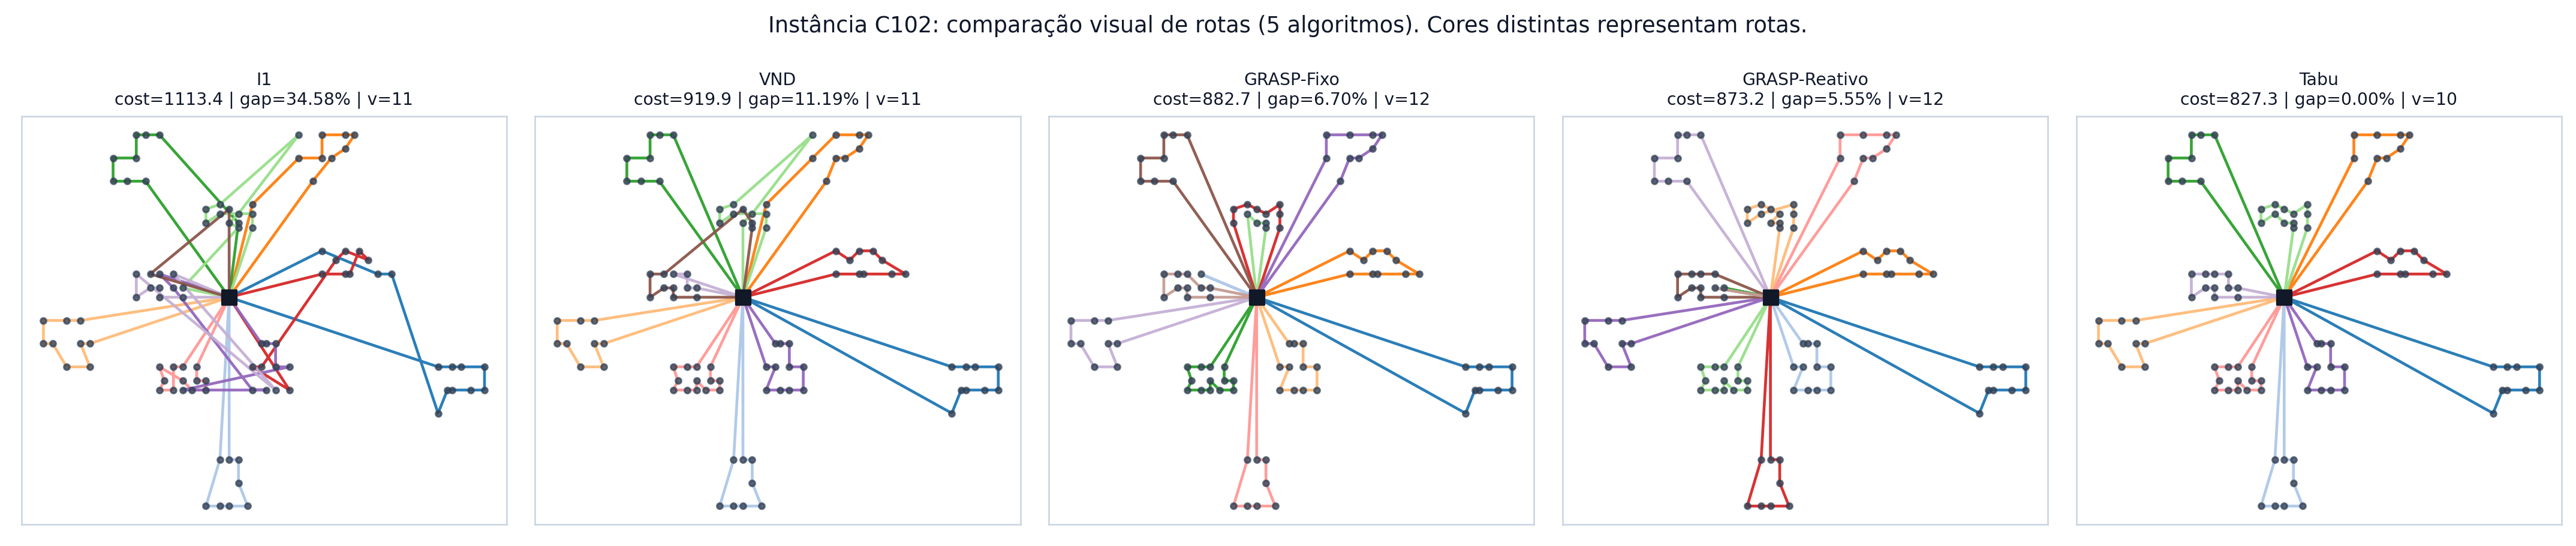
\includegraphics[width=\linewidth]{figs/png/route_compare_C.png}}{\fbox{\parbox{0.9\linewidth}{Figura ausente. Execute \texttt{python3 scripts/build_article_route_panels.py}.}}}
\caption{Família C: instância C102 (ganho vs I1 = 286.1, 25.70\%; distância ao BKS do melhor método = 0.0). Melhor algoritmo nessa instância: \texttt{tabu}. Cada coluna mostra a rota final de um algoritmo na mesma instância.}
\label{fig:route_compare_C}
\end{figure}

\begin{figure}[htbp]
\centering
\IfFileExists{figs/png/route_compare_R.png}{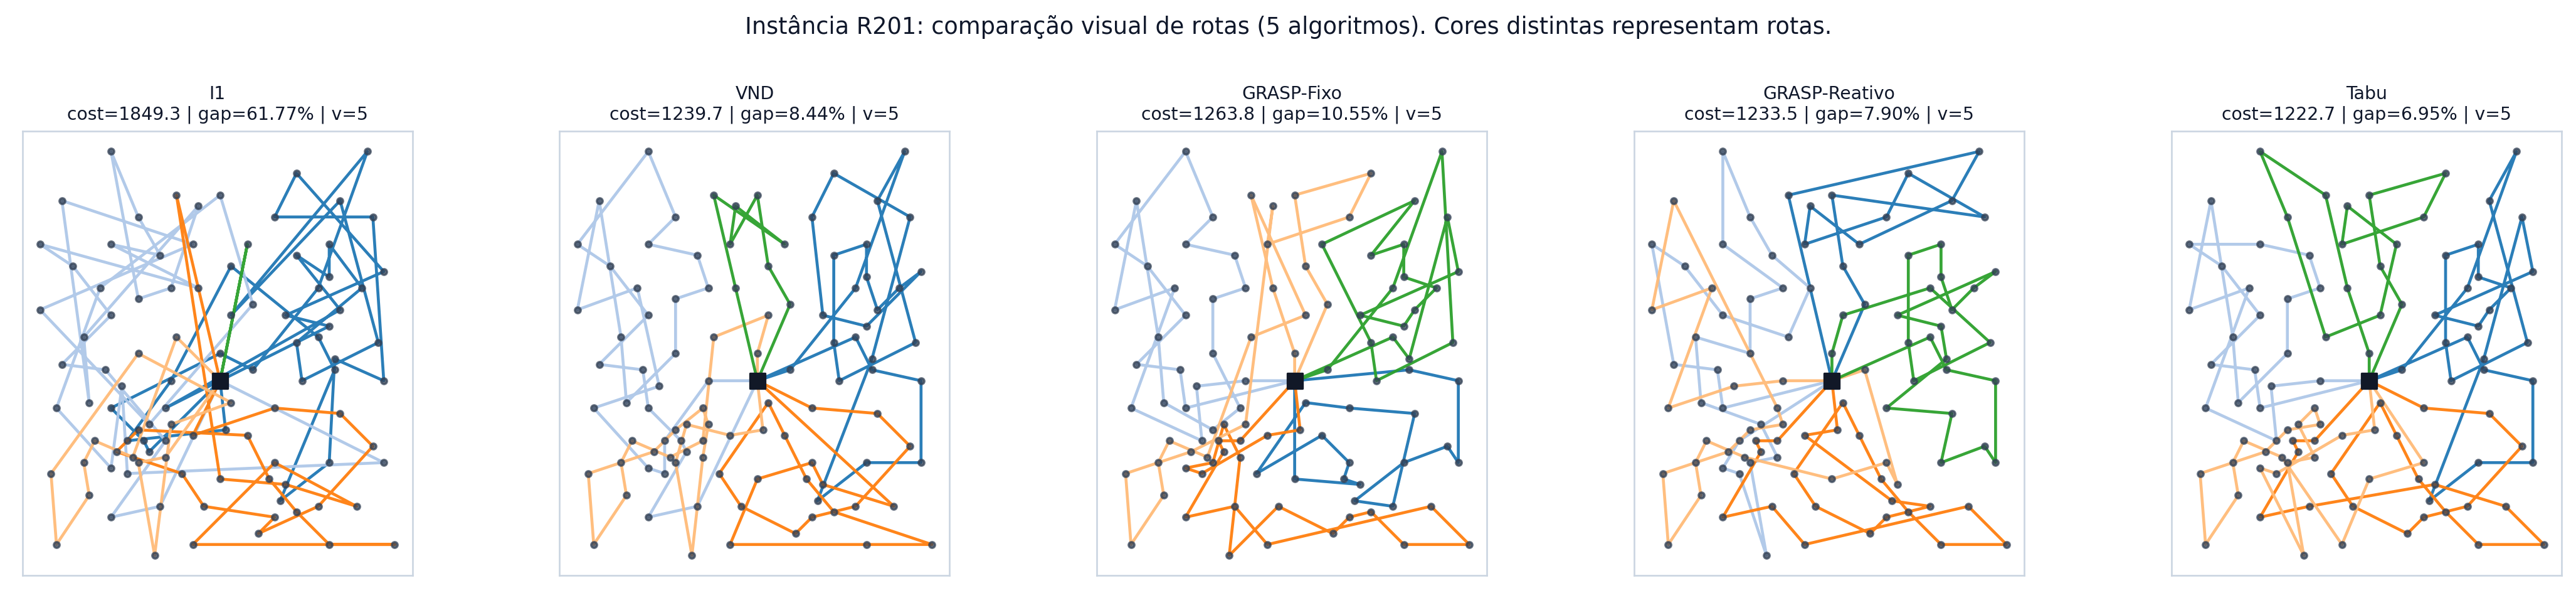
\includegraphics[width=\linewidth]{figs/png/route_compare_R.png}}{\fbox{\parbox{0.9\linewidth}{Figura ausente. Execute \texttt{python3 scripts/build_article_route_panels.py}.}}}
\caption{Família R: instância R201 (ganho vs I1 = 626.6, 33.88\%; distância ao BKS do melhor método = 79.5). Melhor algoritmo nessa instância: \texttt{tabu}. Cada coluna mostra a rota final de um algoritmo na mesma instância.}
\label{fig:route_compare_R}
\end{figure}

\begin{figure}[htbp]
\centering
\IfFileExists{figs/png/route_compare_RC.png}{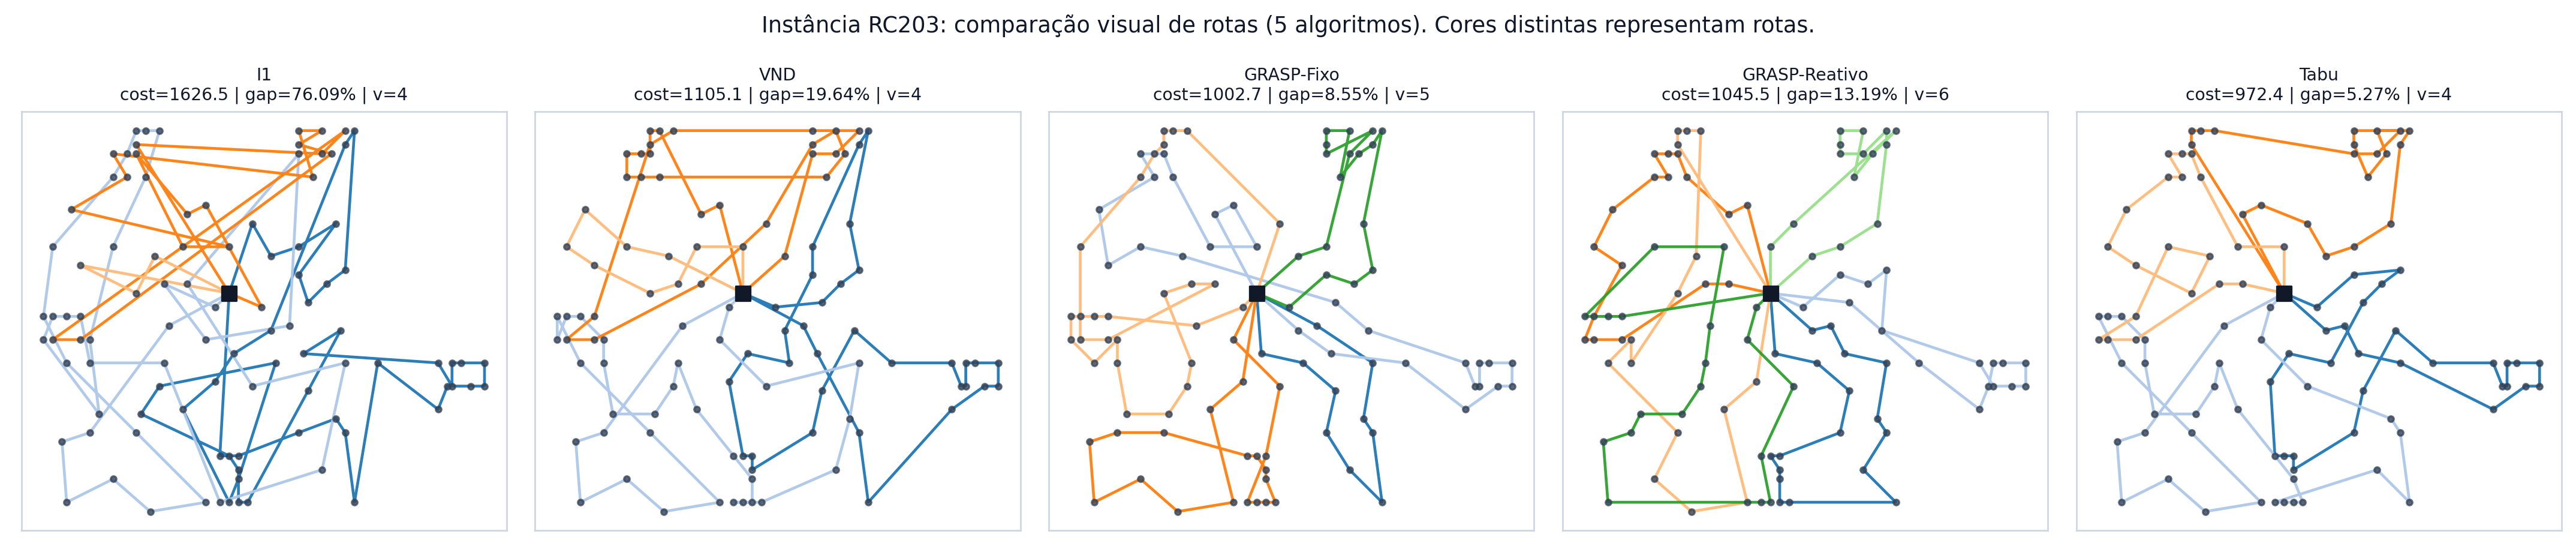
\includegraphics[width=\linewidth]{figs/png/route_compare_RC.png}}{\fbox{\parbox{0.9\linewidth}{Figura ausente. Execute \texttt{python3 scripts/build_article_route_panels.py}.}}}
\caption{Família RC: instância RC203 (ganho vs I1 = 654.1, 40.22\%; distância ao BKS do melhor método = 48.7). Melhor algoritmo nessa instância: \texttt{tabu}. Cada coluna mostra a rota final de um algoritmo na mesma instância.}
\label{fig:route_compare_RC}
\end{figure}

}{
\begin{table}[htbp]
\centering
\caption{Painéis de rotas (pendente de geração).}
\begin{tabular}{lc}
\hline
Status & Observação \\
\hline
Pendente & Execute \texttt{python3 scripts/build\_article\_route\_panels.py}. \\
\hline
\end{tabular}
\end{table}
}
